\section{Results}

\subsection{Results with simple simulation}
The simple simulation is characterized by sensors being spread evenly throughout the map. The rule is that a sensor cannot touch another sensor. The figure below illustrates the success of the fire interpreter. The light green color is where the actual fire is and where the interpreter predicted it to be. Therefore the color of success. The dark green color is area where the interpreter thought it would be fire, but was not. The red parts are the actual fire which the interpreter did not predict.
\begin{figure}[here]
  \centering
      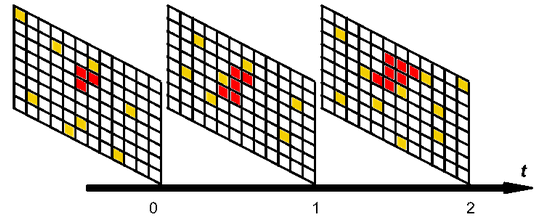
\includegraphics[width=0.5\textwidth]{solution/graphics/timeElapse.png}
  \caption{The fire interpreter saves the sensor data (yellow dots) with \textbf{t}.}
  \label{fig:simple-results}
\end{figure}


\subsection{Results with advanced simulation}